\begin{figure}
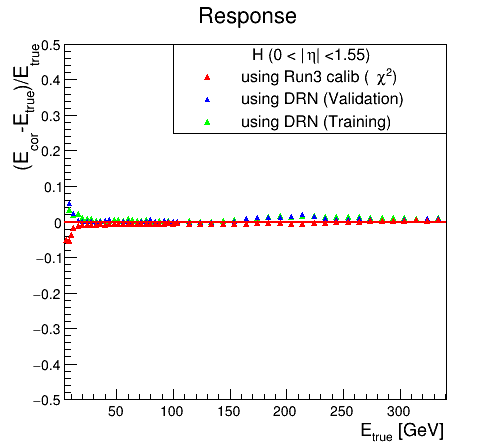
\includegraphics[width=0.495\textwidth]{./plots_pdf/HCAL_plots/Trained_target_ratioflip_0_500_10/pdf/H_barrel/barrel_corrEtaBarrelHcal.png}
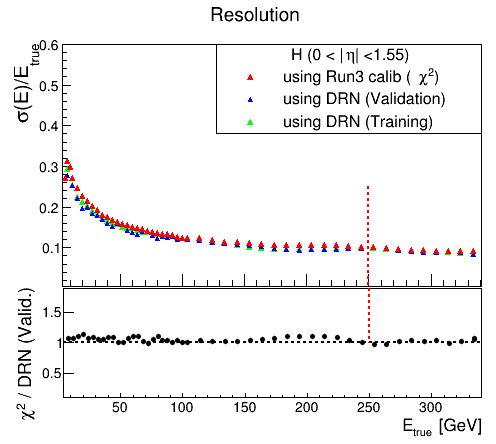
\includegraphics[width=0.495\textwidth]{./plots_pdf/HCAL_plots/Trained_target_ratioflip_0_500_10/pdf/H_barrel/barrel_corrEtaBarrelHcal_reso.png}

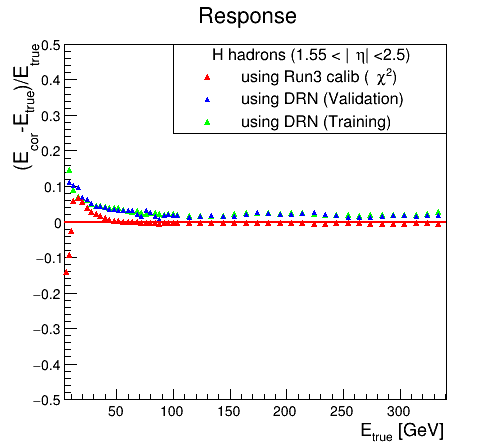
\includegraphics[width=0.495\textwidth]{./plots_pdf/HCAL_plots/Trained_target_ratioflip_0_500_10/pdf/H_ec_in/EC_within_tracker_corrEtaEndcapHcal.png}
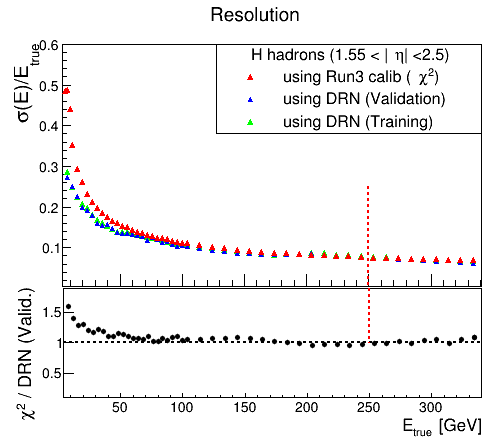
\includegraphics[width=0.495\textwidth]{./plots_pdf/HCAL_plots/Trained_target_ratioflip_0_500_10/pdf/H_ec_in/EC_within_tracker_corrEtaEndcapHcal_reso.png}

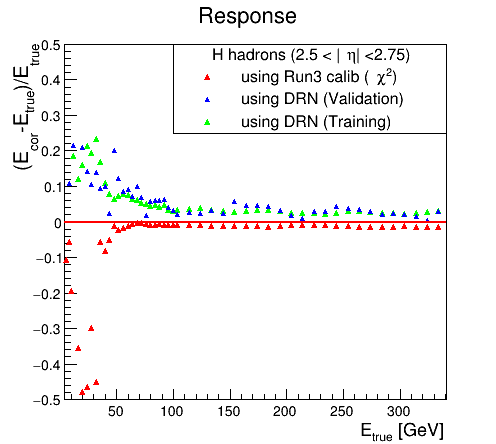
\includegraphics[width=0.495\textwidth]{./plots_pdf/HCAL_plots/Trained_target_ratioflip_0_500_10/pdf/H_ec_out/EC_outside_tracker_corrEtaEndcapHcal.png}
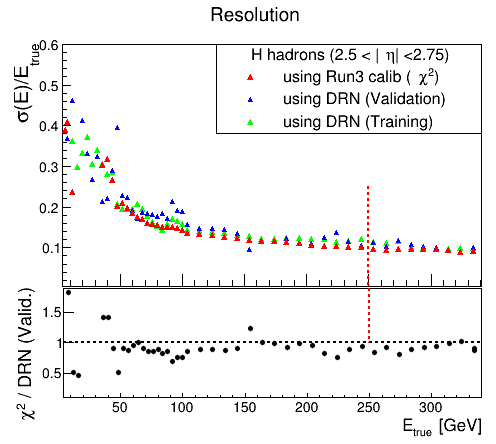
\includegraphics[width=0.495\textwidth]{./plots_pdf/HCAL_plots/Trained_target_ratioflip_0_500_10/pdf/H_ec_out/EC_outside_tracker_corrEtaEndcapHcal_reso.png}

\caption[ Response (resolution) vs \pt of the PF H-hadron cluster - traget log(ratioflip)]{Mean response (resolution) defined by calibrated PF H-hadron clusters using $\chi^{2}$ method (red), DRN modle derived from training samples (green), DRN modle validated on testing samples (blue). (top) barrel, (middle) endcap within tracker, (bottom) endcap outside the tracker. DRN training target is log(ratioflip)}
\label{fig:H_logratioflip}

\end{figure}
